\section{Output Options}
\label{sec:output_options}
The Options tab specifies the working directory, frame, configuration options for the \verb|.emtg| solution file produced when \ac{EMTG} is run and other miscellaneous settings. This tab can also activate a number of additional file outputs which can be useful during the mission planning process. These include an integrated ephemeris file for the spacecraft which can be converted into a \ac{SPICE} SPK (Spacecraft and Planetary Kernel) file as well as maneuver and target specification files providing more detail about each of the maneuvers in the \ac{EMTG} solution. This section covers the available options for \ac{EMTG}'s output files.

    \begin{figure}[H]
        \centering
        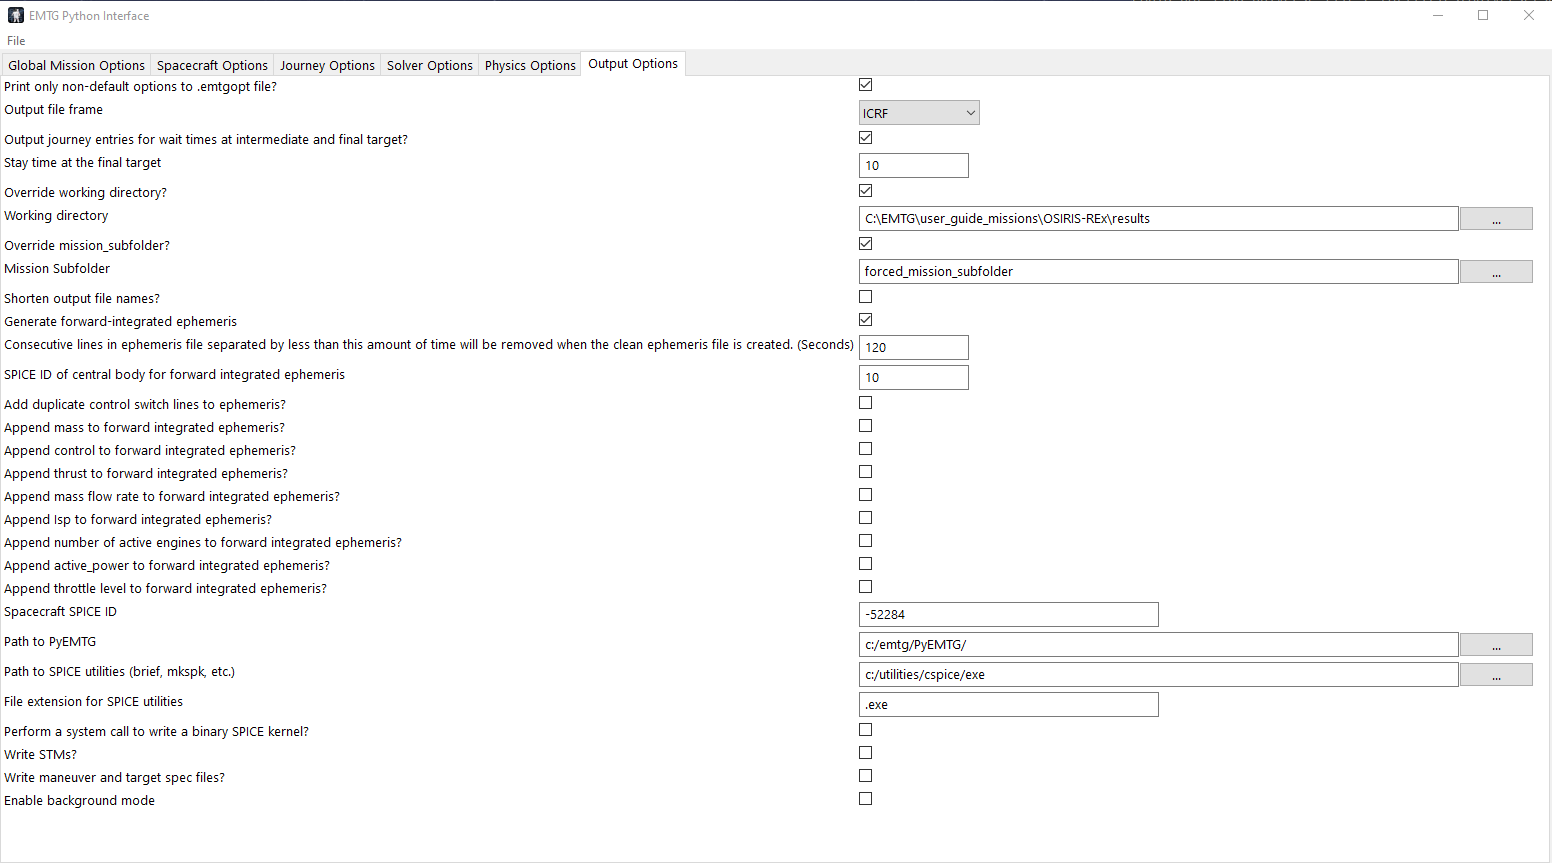
\includegraphics[width=0.95\linewidth]{../../shared_latex_inputs/images/pyemtg_output_options.png}
        \caption{PyEMTG Output Options}
    \end{figure}

\subsection{General Output Options}

    \begin{enumerate}
    \item{\textbf{Print only non-default options to .emtgopt file?:}} Selecting this option will cause PyEMTG to only include options in the \ac{EMTG} Options file that the user has changed from their default values. This can make it easier to review the options file, but only if the user is already familiar with \ac{EMTG}'s default behavior. It is recommended to leave this box unchecked so the full set of options may be easily viewed by users, as some options are only present in the \ac{EMTG} Options file and not in PyEMTG.
    % When learning to use \ac{EMTG} it can be beneficial to leave this box unchecked in order to see all options especially since some options are only present in the \ac{EMTG} Options file and not in PyEMTG.

        \begin{table}[H]
            \hspace{2cm}
            \begin{tabular}{ll}
            Data Type & \verb|bool| \\
            Allowed Values & true, false \\
            Default Value & false \\
            Units & NA
            \end{tabular}
        \end{table}

    \item{\textbf{Output file frame:}} Specify the desired reference frame to be used in the \ac{EMTG} output files. Note that \ac{EMTG}'s basic trajectory plotting tool uses \ac{ICRF}. If another output frame is selected the trajectory plot will not be accurate.
    
        \begin{table}[H]
            \hspace{2cm}
            \begin{tabular}{lp{3cm}}
            Data Type & \verb| (ReferenceFrame) enum| \\
            Allowed Values & \verb|ICRF,|\newline
            \verb|J2000_BCI,| \newline 
            \verb|J2000_BCF, |\newline
            \verb|TrueOfDate_BCI,| \newline 
            \verb|TrueOfDate_BCF,| \newline 
            \verb|PrincipleAxes,| \newline
            \verb|Topocentric,| \newline
            \verb|Polar,| \newline
            \verb|SAM,| \newline
            \verb|ObjectReferenced| \\
            Default Value & \verb|ICRF|\\
            \end{tabular}
        \end{table}

    \item{\textbf{Output journey entries for wait times at intermediate and final target?:}} Selecting this option will cause \ac{EMTG} to include entries in the output \verb|.emtg| file depicting the spacecraft waiting at an ephemeris body prior to departure as in Figure \ref{fig:journey_wait_entries}. Normally these entries are skipped and there will be a gap between the spacecraft's arrival at an ephemeris body and its departure at the start of the next Journey. Selecting this option also activates and reveals an option to stay at the final target ephemeris body.
        
        \begin{table}[H]
            \hspace{2cm}
            \begin{tabular}{ll}
            Data Type & \verb|bool| \\
            Allowed Values & true, false \\
            Default Value & false \\
            Units & NA
            \end{tabular}
        \end{table}

        \begin{figure}[H]
            \centering
            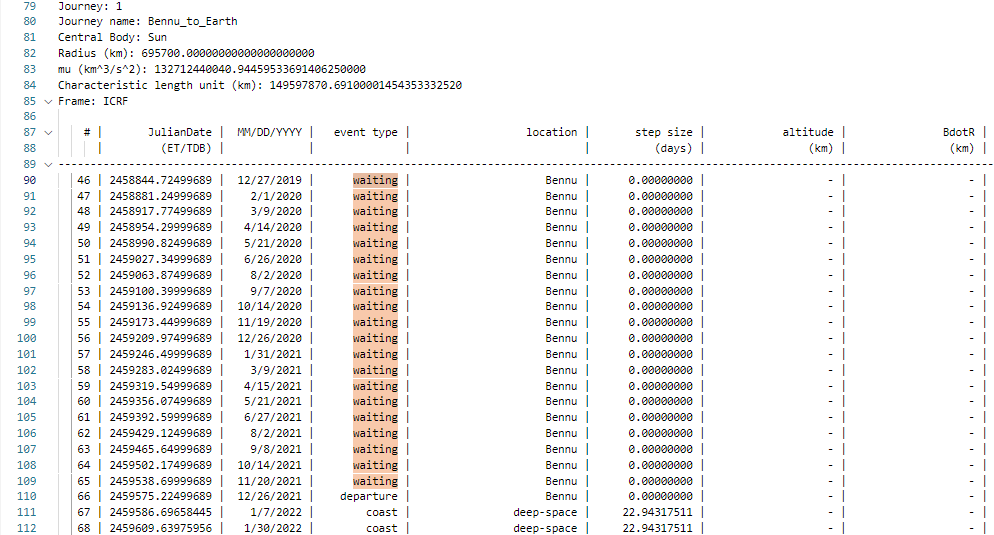
\includegraphics[width=0.95\linewidth]{../../shared_latex_inputs/images/output_wait_entries.png}
            \caption{Journey Wait Entries}
            \label{fig:journey_wait_entries}
        \end{figure}



    \item{\textbf{Stay time at the final target:}} This setting causes \ac{EMTG} to add Journey entries in the output \verb|.emtg| file at the final mission target for the specified number of days. Only active when the ``Output journey entries for wait times'' option is selected.
        
        \begin{table}[H]
            \hspace{2cm}
            \begin{tabular}{ll}
            Data Type & \verb|double| \\
            Allowed Values & 0 $<$ Real $<$ $\infty$ \\
            Default Value & 0.0 \\
            Units & days
            \end{tabular}
        \end{table}

    \item{\textbf{Override working directory:}} By default when \ac{EMTG} is run it will create a new run directory (also known as the mission subfolder) in the \verb|EMTG_v9_results| folder in the \ac{EMTG} install location named using the mission name in the Global Options tab followed by the current date and time. This behavior can be changed by selecting this option and specifying the output directory in the ``Working directory'' option activated and revealed by this setting. The provided path may be either relative to the PyEMTG executable or absolute. It is recommended to always use absolute paths.
    
        \begin{table}[H]
            \hspace{2cm}
            \begin{tabular}{ll}
            Data Type & \verb|bool| \\
            Allowed Values & true, false \\
            Default Value & false \\
            Units & NA
            \end{tabular}
        \end{table}

        \item{\textbf{Working directory:}} Specifies the path to the new working directory.
        
            \begin{table}[H]
                \hspace{2cm}
                \begin{tabular}{ll}
                Data Type & \verb|string| \\
                Default Value & ``..//\ac{EMTG}\_v9\_Results'' \\
                \end{tabular}
            \end{table}

    \item{\textbf{Override mission subfolder?:}} This option changes the default run directory naming convention of the mission name followed by the current date and time. This option also activates and reveals the ``Mission subfolder'' option allowing the user to specify a custom directory name which will be created at runtime in the working directory specified earlier.
    
        \begin{table}[H]
            \hspace{2cm}
            \begin{tabular}{ll}
            Data Type & \verb|bool| \\
            Allowed Values & true, false \\
            Default Value & false \\
            Units & NA
            \end{tabular}
        \end{table}

    \item{\textbf{Mission subfolder:}} Specifies the new mission subfolder (run directory) name. This subfolder is created within the working directory. If there are any pre-existing files of the same name, they will be overwritten.
    
        \begin{table}[H]
            \hspace{2cm}
            \begin{tabular}{ll}
            Data Type & \verb|string| \\
            Default Value & ``forced\_mission\_subfolder'' \\
            \end{tabular}
        \end{table}

    \item{\textbf{Shorten output file names?:}} Removes additional Journey information from the name of the \verb|.emtg| output file and uses just the mission name as the filename.
    
        \begin{table}[H]
            \hspace{2cm}
            \begin{tabular}{ll}
            Data Type & \verb|bool| \\
            Allowed Values & true, false \\
            Default Value & true \\
            Units & NA
            \end{tabular}
        \end{table}

    \item{\textbf{Write STMs?:}} Creates state transition matrix \verb|.stm| output files for every Journey Phase along with a set of \verb|.stm_description| files containing the row and column variable names.

        \begin{table}[H]
            \hspace{2cm}
            \begin{tabular}{ll}
            Data Type & \verb|bool| \\
            Allowed Values & true, false \\
            Default Value & false \\
            Units & NA
            \end{tabular}
        \end{table}

    \item{\textbf{Write maneuver and target spec files?:}} These files provide detailed information for each maneuver in the mission and can be used when converting an \ac{EMTG} trajectory to a final, flight-ready trajectory. The Maneuver Specification file lists the epoch, thrust direction, margin, duration, DV, and other information about each maneuver. The Target Specification file  stores the epoch, frame, central body, and state vector (position, velocity, mass), and B-plane coordinates (if applicable) associated with the target for each maneuver.
    
        \begin{table}[H]
            \hspace{2cm}
            \begin{tabular}{ll}
            Data Type & \verb|bool| \\
            Allowed Values & true, false \\
            Default Value & false \\
            Units & NA
            \end{tabular}
        \end{table}
    
    \item{\textbf{Enable background mode:}} Disables almost all terminal output when running \ac{EMTG}.
    
        \begin{table}[H]
            \hspace{2cm}
            \begin{tabular}{ll}
            Data Type & \verb|bool| \\
            Allowed Values & true, false \\
            Default Value & false \\
            Units & NA
            \end{tabular}
        \end{table}

\end{enumerate}


\subsection{Ephemeris Output Options}
\label{sec:output_ephemeris_options}

\ac{EMTG} can produce a forward integrated Ephemeris Table or timeseries of the spacecraft's position, velocity and other information as a text file. On the Output Options tab in PyEMTG select ``Generate forward-integrated ephemeris.'' This will reveal additional options to configure the ephemeris table output. In addition to spacecraft position and velocity which are written by default, users may select to show spacecraft mass, control, thrust, mass flow rate, ISP, and other engine parameters. 

\noindent The forward-integrated ephemeris can be used to create a binary \ac{SPICE} kernel \verb|.bsp| file for use with other software through the use of a short Python script \verb|bspwriter.py| which is automatically created in the output directory when the ``Generate forward-integrated ephemeris option'' is active. The \verb|bspwriter.py| script also ``cleans'' the ephemeris removing duplicate entries and enforcing the timestep resolution set by the ``Consecutive lines in ephemeris file separated by less than...'' option described below.

\begin{alertbox}{\emtgknownissue{Issue with forward-integrated ephemeris.}{Forward-integrated Ephemeris Issue}}
% \begin{alertbox}{Forward-integrated Ephemeris Issue}
    \noindent If the \ac{EMTG} mission (final Journey) ends with an impulsive maneuver such as a capture burn at a body, the final line of the ephemeris may not contain the impulsive delta-v. Instead the ephemeris file will show two repeated entries at the final epoch of the mission. The second of these entries is intended to contain the spacecraft state immediately following the final impulsive delta-v. This typically would only be an issue at initial stages of mission design prior to the conversion to finite burns. If desired, the final impulsive maneuver can be made to appear by adding another ``fake'' Journey to the end of the mission. 



    \begin{figure}[H]
        \centering
        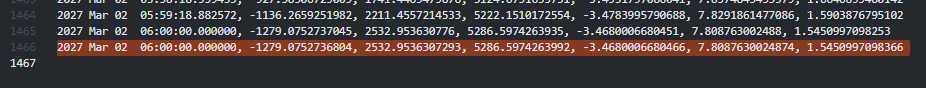
\includegraphics[width=0.95\linewidth]{../../shared_latex_inputs/images/ephemeris_dv_bug.png}
        \caption{Forward-integrated Ephemeris Final DV Issue}
    \end{figure}

\noindent The example Journey options below shows one configuration of an additional coast Journey lasting 0.01 days which can be added as a final Journey to trigger the post-impulsive delta-v state to appear in the forward-integrated ephemeris. This method should be used with the ``evaluate trialX'' solver mode rather than the \ac{NLP} or \ac{MBH} modes to avoid the Journey impacting the overall mission or solution feasibility.

    \begin{figure}[H]
        \centering
        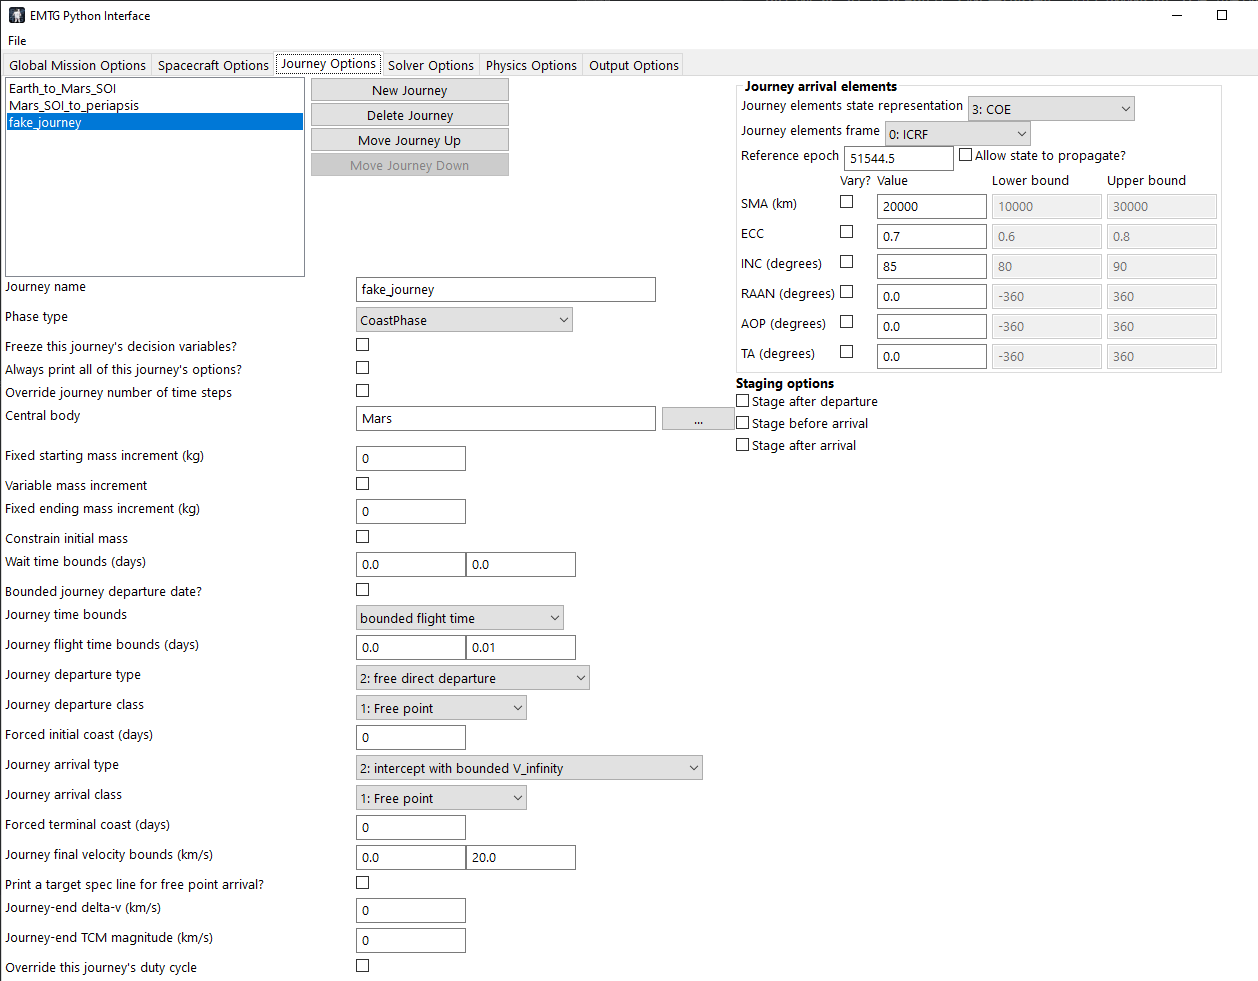
\includegraphics[width=0.95\linewidth]{../../shared_latex_inputs/images/extra_journey_options.png}
        \caption{Example Extra Journey Configuration}
    \end{figure}

\end{alertbox}


\begin{enumerate}

\item{\textbf{Generate forward-integrated ephemeris:}} Turns on creation of the forward-integrated ephemeris file in the working directory specified above. Reveals the additional options below.

    \begin{table}[H]
        \hspace{2cm}
        \begin{tabular}{ll}
        Data Type & \verb|bool| \\
        Allowed Values & true, false \\
        Default Value & false \\
        Units & NA
        \end{tabular}
    \end{table}


\item{\textbf{Consecutive lines in ephemeris file separated by less than this amount of time will be removed:}} Set the timestep resolution in the forward-integrated ephemeris file. Can be overridden at the Journey-level see Section \ref{sec:journey_options}.

    \begin{table}[H]
        \hspace{2cm}
        \begin{tabular}{ll}
        Data Type & \verb|double| \\
        Allowed Values & 1.0E-5 $<$ Real $<$ $\infty$ \\
        Default Value & 120 \\
        Units & seconds
        \end{tabular}
    \end{table}

\item{\textbf{\ac{SPICE} ID of central body for forward integrated ephemeris:}} The forward-integrated ephemeris can be output using any body in the Universe as a central body by setting this option to the appropriate \ac{SPICE} ID. The body must be present in one of the \ac{SPICE} kernels provided in the \verb|ephemeris_files| directory located with the mission Universe files.  
% #?? does this work with bodies provided as orbital elements instead of spice kernels?

    \begin{table}[H]
        \hspace{2cm}
        \begin{tabular}{ll}
        Data Type & \verb|integer| \\
        Allowed Values & $-\infty$ $<$ Real $<$ $\infty$ \\
        Default Value & 10 \\
        Units & NA
        \end{tabular}
    \end{table}

\item{\textbf{Add duplicate control switch lines to ephemeris?:}} This option was used prior to the maneuver spec files and will be removed in a future release. 


\item{\textbf{Append mass to forward integrated epehemeris?:}} Add spacecraft mass in kilograms as an additional column in the forward-integrated ephemeris.
    \begin{table}[H]
        \hspace{2cm}
        \begin{tabular}{ll}
        Data Type & \verb|bool| \\
        Allowed Values & true, false \\
        Default Value & false \\
        Units & NA
        \end{tabular}
    \end{table}

\item{\textbf{Append control to forward integrated epehemris?:}} Add thrust direction unit vector as additional columns in the forward-integrated ephemeris.
    \begin{table}[H]
        \hspace{2cm}
        \begin{tabular}{ll}
        Data Type & \verb|bool| \\
        Allowed Values & true, false \\
        Default Value & false \\
        Units & NA
        \end{tabular}
    \end{table}

\item{\textbf{Append thrust to forward integrated epehemris?:}} Add thrust in Newtons as an additional column in the forward-integrated ephemeris.
    \begin{table}[H]
        \hspace{2cm}
        \begin{tabular}{ll}
        Data Type & \verb|bool| \\
        Allowed Values & true, false \\
        Default Value & false \\
        Units & NA
        \end{tabular}
    \end{table}

\item{\textbf{Append mass flow rate to forward integrated epehemeris?:}} Add mass flow rate in kilograms/second as an additional column in the forward-integrated ephemeris.
    \begin{table}[H]
        \hspace{2cm}
        \begin{tabular}{ll}
        Data Type & \verb|bool| \\
        Allowed Values & true, false \\
        Default Value & false \\
        Units & NA
        \end{tabular}
    \end{table}
\item{\textbf{Append Isp to forward integrated ephemeris?:}} Add Isp in seconds as an additional column in the forward-integrated ephemeris.
    \begin{table}[H]
        \hspace{2cm}
        \begin{tabular}{ll}
        Data Type & \verb|bool| \\
        Allowed Values & true, false \\
        Default Value & false \\
        Units & NA
    \end{tabular}
\end{table}
\item{\textbf{Append number of active engines to forward integrated ephemris?:}} Add number of active engines as an additional column in the forward-integrated ephemeris.
    \begin{table}[H]
        \hspace{2cm}
        \begin{tabular}{ll}
        Data Type & \verb|bool| \\
        Allowed Values & true, false \\
        Default Value & false \\
        Units & NA
        \end{tabular}
    \end{table}

\item{\textbf{Append active\_power to forward integrated ephemeris?:}} Add active spacecraft power in kiloWatts as an additional column in the forward-integrated ephemeris.
    \begin{table}[H]
        \hspace{2cm}
        \begin{tabular}{ll}
        Data Type & \verb|bool| \\
        Allowed Values & true, false \\
        Default Value & false \\
        Units & NA
        \end{tabular}
    \end{table}

\item{\textbf{Append throttle level to forward integrated ephemeris?:}} Add throttle level as an additional column in the forward-integrated ephemeris.
    \begin{table}[H]
        \hspace{2cm}
        \begin{tabular}{ll}
        Data Type & \verb|bool| \\
        Allowed Values & true, false \\
        Default Value & false \\
        Units & NA
        \end{tabular}
    \end{table}

\item{\textbf{Spacecraft \ac{SPICE} ID:}} \ac{SPICE} ID to be used when creating a binary \ac{SPICE} kernel. It's recommended to use a negative integer. By convention, spacecraft \ac{SPICE} IDs are negative integer values to avoid ID collision with a body. \ac{EMTG} does not enforce this requirement, but other software which reads \ac{SPICE} kernels may. 

    \begin{table}[H]
        \hspace{2cm}
        \begin{tabular}{ll}
        Data Type & \verb|integer| \\
        Allowed Values & $-\infty$ $<$ Real $<$ $\infty$ \\
        Default Value & -52284 \\
        Units & NA
        \end{tabular}
    \end{table}

\item{\textbf{Path to PyEMTG:}} Path to the directory containing the \verb|PyEMTG.py| file.

    \begin{table}[H]
        \hspace{2cm}
        \begin{tabular}{ll}
        Data Type & \verb|string| \\
        Default Value & ``c:/emtg/PyEMTG/'' \\
        \end{tabular}
    \end{table}

\item{\textbf{Path to \ac{SPICE} utilities:}} Path to the directory containing the \ac{SPICE} executable utilities.

    \begin{table}[H]
        \hspace{2cm}
        \begin{tabular}{ll}
        Data Type & \verb|string| \\
        Default Value & ``c:/utilities/cspice/exe'' \\
        \end{tabular}
    \end{table}

\item{\textbf{File extension for \ac{SPICE} utilities:}} File extension for the \ac{SPICE} executable utilities.

    \begin{table}[H]
        \hspace{2cm}
        \begin{tabular}{ll}
        Data Type & \verb|string| \\
        Default Value & ``.exe'' \\
        \end{tabular}
    \end{table}

\item{\textbf{Perform a system call to write a binary \ac{SPICE} kernel?:}} When forward-integrated epehemeris is generated a short Python script, \verb|bspwriter.py|, is also created in the output directory which when executed will create the \ac{SPICE} kernel \verb|.bsp| file and a cleaned copy of the \verb|.ephemeris| file. Selecting this option will automatically execute the \verb|bspwriter.py| script. Alternatively users may execute the script themselves.

    \begin{table}[H]
        \hspace{2cm}
        \begin{tabular}{ll}
        Data Type & \verb|bool| \\
        Allowed Values & true, false \\
        Default Value & false \\
        Units & NA
        \end{tabular}
    \end{table}

\end{enumerate}





